\documentclass[17pt, t, lualatex]{beamer}



\title{\LARGE Ejercicios del profe: Colas 2025-1}
\date{\today}
\institute[UJTL]{Universidad Jorge Tadeo Lozano - Semillero de Programación Competitiva}
\author{Ludwig Alvarado Becerra}

\usepackage{amsmath, amssymb, mathtools}
\usepackage[spanish]{babel}
\usepackage{biblatex}
\usepackage{hyperref}
\usepackage{xurl}
\usepackage{cancel}
\usepackage{svg}
\usepackage{listings}
\usepackage{xcolor}
\usepackage{array}

% Define colors
\definecolor{codebg}{rgb}{0.95,0.95,0.95}
\definecolor{commentcolor}{rgb}{0.0,0.5,0.0}
\definecolor{keywordcolor}{rgb}{0.0,0.0,0.8}
\definecolor{stringcolor}{rgb}{0.58,0.0,0.82}

% Define C++ style
\lstdefinestyle{cppstyle}{
    language=C++,
    backgroundcolor=\color{codebg},
    basicstyle=\ttfamily\small,
    keywordstyle=\color{keywordcolor}\bfseries,
    stringstyle=\color{stringcolor},
    commentstyle=\color{commentcolor}\itshape,
    numbers=left,
    numberstyle=\tiny\color{gray},
    stepnumber=1,
    numbersep=8pt,
    showspaces=false,
    showstringspaces=false,
    showtabs=false,
    frame=single,
    tabsize=4,
    breaklines=true,
    breakatwhitespace=true,
    captionpos=b,
    morekeywords={endl,pop}
}

% Define a new inline command using your cppstyle
\newcommand{\cppinline}[1]{\lstinline[style=cppstyle]!#1!}


\addbibresource{referencias.bib}  % Make sure your .bib file is correctly named


\addbibresource{referencias.bib}

% Probably load as late as possible
% Other options are
% - engine=pdflatex to compile in pdfLaTeX (with different fonts),
% - mathshape=rm to use serif font for math,
% - mathsahpe=custom to not set any math font (so that you can define your own math fonts)
\usetheme[engine=lualatex, mathshape=sf, fontdir=kthpq-files/fonts/Figtree/]{kthpq}
\setmonofont{Bitstream Vera Sans Mono}[Scale=.9]

% Custom colors (see beamercolorthemecustom.sty for more details)
% \usecolortheme{custom}

% Modify the headline template: KTH-full, KTH-section-only, or KTH-frametitle-only.
% \setbeamertemplate{headline}[KTH-full]

% Custom footline
% \setfootline{left}{center}{right}

\begin{document}

\inserttitlepage

\section{Problema 2}

\insertsectionpage


\begin{frame}
  \frametitle{Problema 2}

  Dada una $\mathbf{cola}$ y un número $\mathbf{k}$, invierte el orden de los primeros $\mathbf{k}$ elementos de la $\mathbf{cola}$. Si $\mathbf{k}$ es mejor que $\mathbf{0}$, si $\mathbf{k}$ excede el tamaño de la $\mathbf{cola}$ o si la $\mathbf{cola}$ está vacía, se devuelve $\mathbf{NULL}$. De lo contrario, se devuelve la $\mathbf{cola}$ modificada.

  \textbf{Restricciones}

  \begin{itemize}
    \item $0 \leq cola.length \leq 10^{3}$
    \item $10^{-3} \leq cola[i] \leq 10^{3}$
    \item $10^{-3} \leq k \leq 10^{3}$
  \end{itemize}

\end{frame}

\begin{frame}
  \frametitle{Problema 2 | Tests}

  \begin{table}[h]
  \centering
  \begin{tabular}{|>{\centering\arraybackslash}p{0.4\textwidth}|>{\centering\arraybackslash}p{0.4\textwidth}|}
    \hline
    \textbf{Entrada} & \textbf{Salida} \\ \hline
    $cola = [1, 2, 3, -4, 5, 6, 7, 8, 9, 10] \quad k = 5$ & $[5, -4, 3, 2, 1, 6, 7, 8, 9, 10]$ \\ \hline
    $cola = [10, -20, 30, 40, -50, 60, 70, 80] \quad k = 3$ & $[30, -20, 10, 40, -50, 60, 70, 80]$ \\ \hline
    $cola = [5, 6, 12, 5, 2, 7, 3] \quad k = 10$ & NULL \\ \hline
    $cola = [43, 5, 12, 4, 9, 6, 5] \quad k = -5$ & NULL \\ \hline
  \end{tabular}
\end{table}

\end{frame}

\begin{frame}
  \frametitle{Test 1}

  \begin{figure}[h]
    \centering
    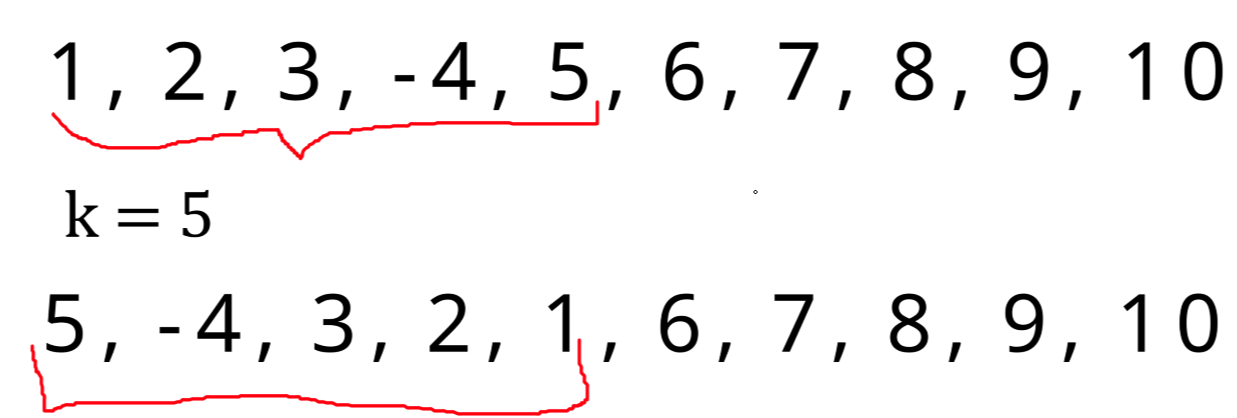
\includegraphics[width=\textwidth]{img/fig1.png}
  \end{figure}

\end{frame}



\section{Solución}

\insertsectionpage



\begin{frame}
  \frametitle{Prerrequisitos}

  \begin{itemize}
    \item Se utiliza un algoritmo para invertir una lista enlazada.
    \item Ejercicio recomendado: \url{https://leetcode.com/problems/reverse-linked-list/description/}
    \item Solución explicada del ejercicio recomendado en: \url{https://github.com/ProgramacionCompetitivaUTADEO/Estructuras-De-Datos/tree/main/C\%2B\%2B/LinkedList/Ejercicios/LC206ReverseLinkedList}
  \end{itemize}

\end{frame}


\begin{frame}
  \frametitle{Diagrama de flujo}


  \begin{figure}[h]
    \centering
    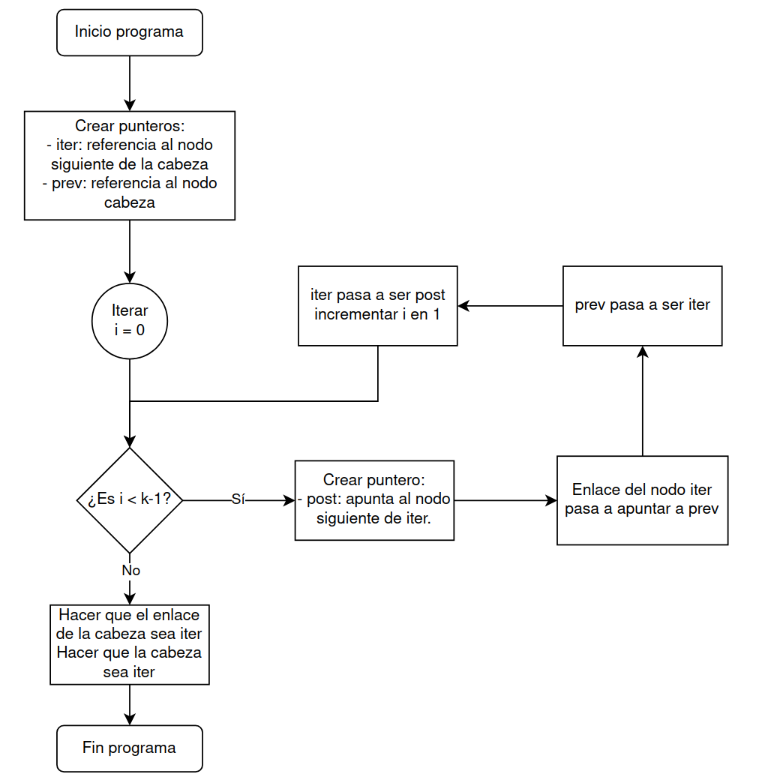
\includegraphics[width=0.4\textwidth]{img/fig2.png}
  \end{figure}


\end{frame}

\begin{frame}
  \frametitle{Funcionamiento del algoritmo}

  \textbf{Cola inicial}

  \begin{figure}[h]
    \centering
    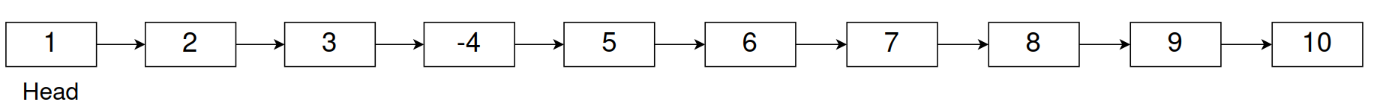
\includegraphics[width=\textwidth]{img/fig3.png}
  \end{figure}

  Inicializar los punteros \cppinline{iter} y \cppinline{prev}

  \begin{figure}[h]
    \centering
    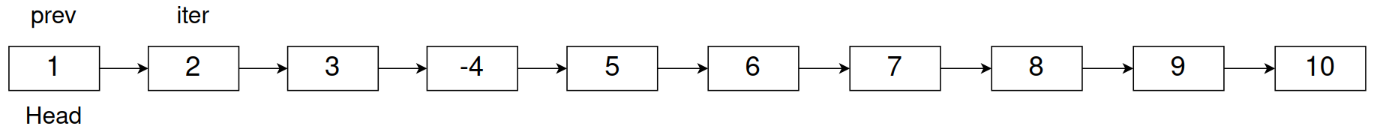
\includegraphics[width=\textwidth]{img/fig4.png}
  \end{figure}


\end{frame}

\begin{frame}
  \frametitle{Funcionamiento del algoritmo}

  \textbf{Inicia el bucle} $i = 0$, condición $i < k-1$. $k = 5$.

  \begin{figure}[h]
    \centering
    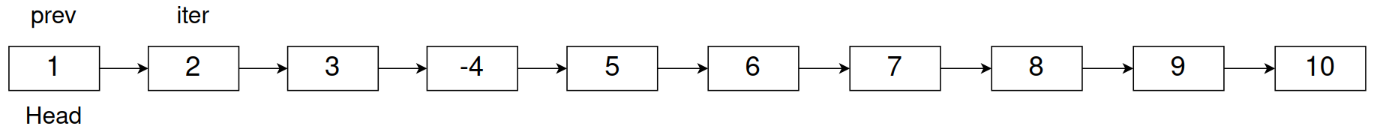
\includegraphics[width=\textwidth]{img/fig4.png}
  \end{figure}

  Crear \cppinline{post} que sea el nodo al que apunta \cppinline{iter}

  \begin{figure}[h]
    \centering
    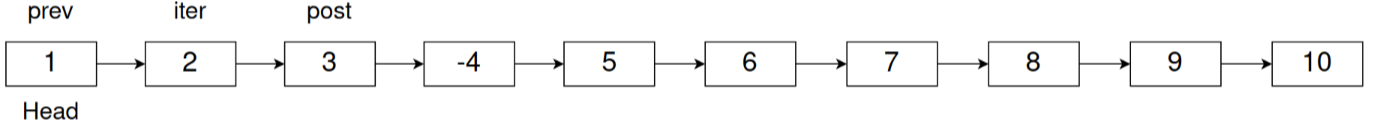
\includegraphics[width=\textwidth]{img/fig5.png}
  \end{figure}


\end{frame}

\begin{frame}
  \frametitle{Funcionamiento del algoritmo}

  Hacer que el nodo \cppinline{iter} apunte al nodo \cppinline{prev}

  \begin{figure}[h]
    \centering
    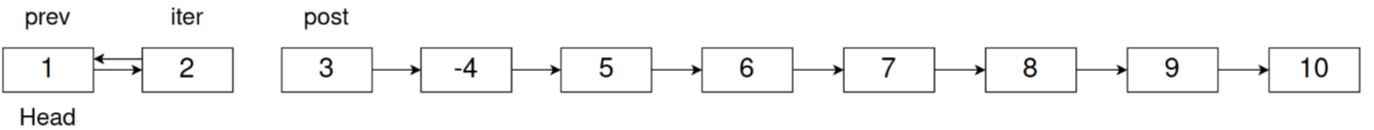
\includegraphics[width=\textwidth]{img/fig6.png}
  \end{figure}

  Mover \cppinline{prev} a \cppinline{iter}

  \begin{figure}[h]
    \centering
    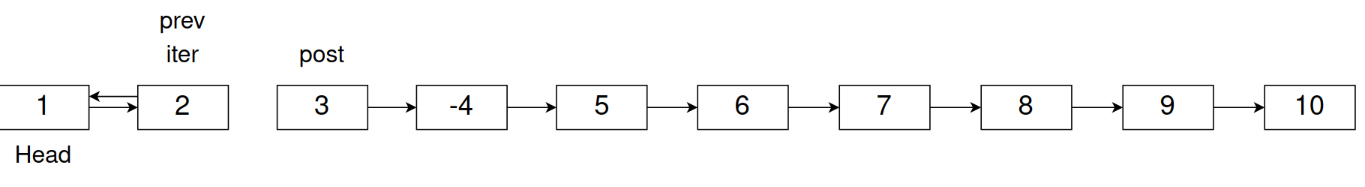
\includegraphics[width=\textwidth]{img/fig7.png}
  \end{figure}


\end{frame}

\begin{frame}
  \frametitle{Funcionamiento del algoritmo}

  Mover \cppinline{iter} a \cppinline{post}.

  \begin{figure}[h]
    \centering
    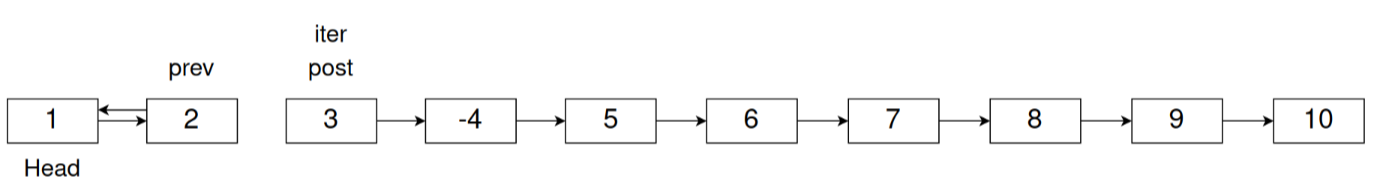
\includegraphics[width=\textwidth]{img/fig8.png}
  \end{figure}

  $i = 1$, condición $i < k-1$. $k = 5$. Crear \cppinline{post} que sea el nodo al que apunta \cppinline{iter}

  \begin{figure}[h]
    \centering
    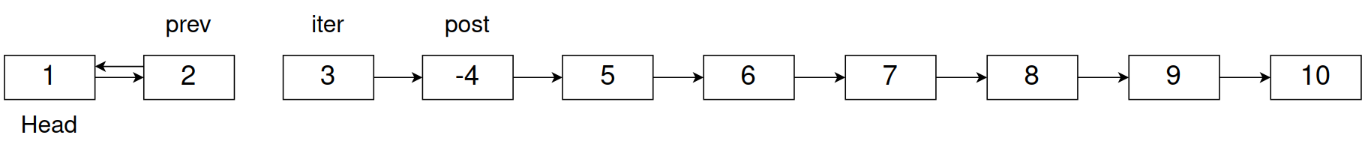
\includegraphics[width=\textwidth]{img/fig9.png}
  \end{figure}


\end{frame}

\begin{frame}
  \frametitle{Funcionamiento del algoritmo}

  Hacer que el nodo \cppinline{iter} apunte al nodo \cppinline{prev}

  \begin{figure}[h]
    \centering
    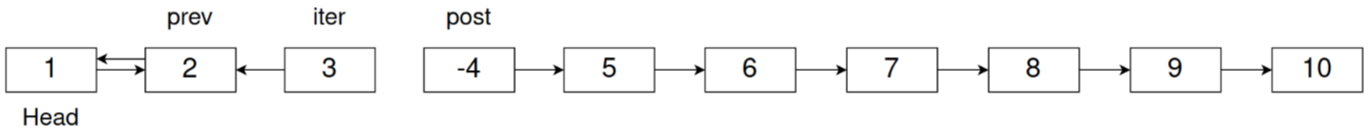
\includegraphics[width=\textwidth]{img/fig10.png}
  \end{figure}

  Mover \cppinline{prev} a \cppinline{iter}

  \begin{figure}[h]
    \centering
    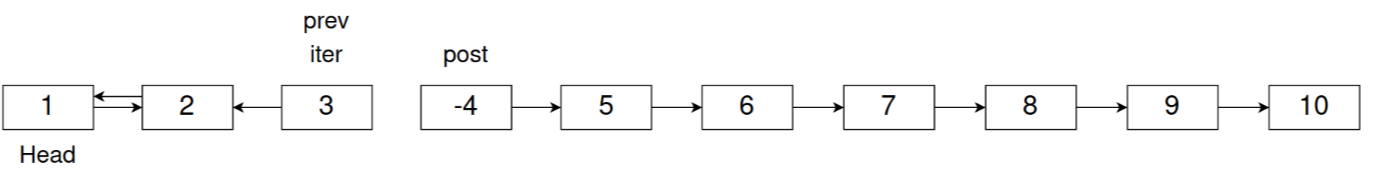
\includegraphics[width=\textwidth]{img/fig11.png}
  \end{figure}


\end{frame}

\begin{frame}
  \frametitle{Funcionamiento del algoritmo}

  Mover \cppinline{iter} a \cppinline{post}

  \begin{figure}[h]
    \centering
    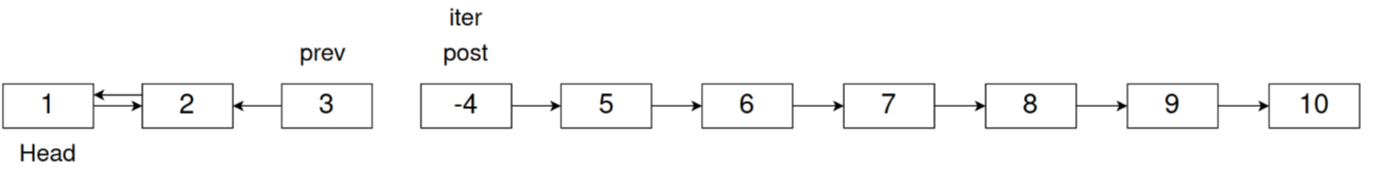
\includegraphics[width=\textwidth]{img/fig12.png}
  \end{figure}

  $i = 2$, condición $i < k-1$. $k = 5$. Crear \cppinline{post} que sea el nodo al que apunta \cppinline{iter}

  \begin{figure}[h]
    \centering
    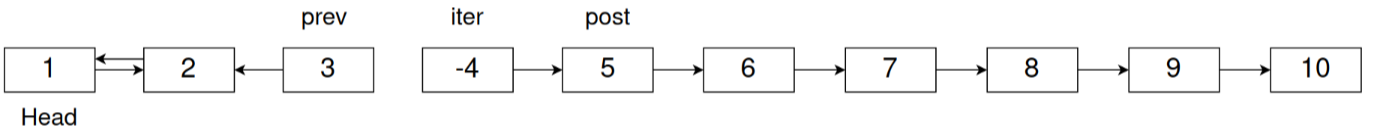
\includegraphics[width=\textwidth]{img/fig13.png}
  \end{figure}

\end{frame}

\begin{frame}
  \frametitle{Funcionamiento del algoritmo}

  Hacer que el nodo \cppinline{iter} apunte al nodo \cppinline{prev}

  \begin{figure}[h]
    \centering
    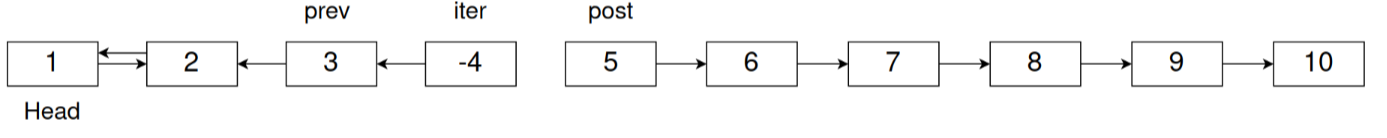
\includegraphics[width=\textwidth]{img/fig14.png}
  \end{figure}

  Mover \cppinline{prev} a \cppinline{iter}

  \begin{figure}[h]
    \centering
    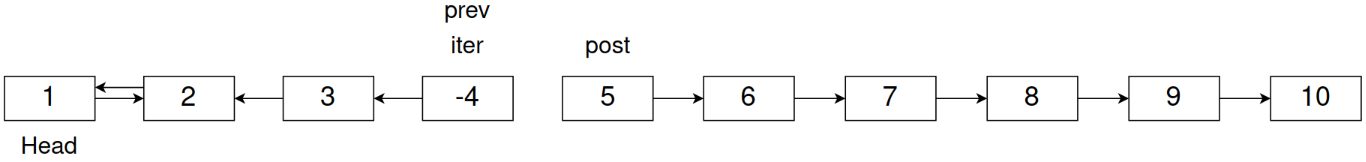
\includegraphics[width=\textwidth]{img/fig15.png}
  \end{figure}

\end{frame}

\begin{frame}
  \frametitle{Funcionamiento del algoritmo}

  Mover \cppinline{iter} a \cppinline{post}

  \begin{figure}[h]
    \centering
    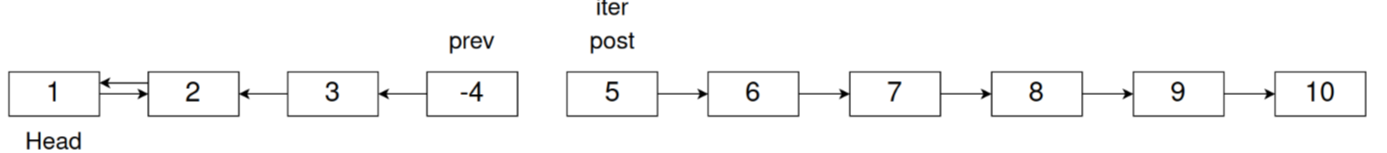
\includegraphics[width=\textwidth]{img/fig16.png}
  \end{figure}

  $i = 3$, condición $i < k-1$. $k = 5$. Crear \cppinline{post} que sea el nodo al que apunta \cppinline{iter}

  \begin{figure}[h]
    \centering
    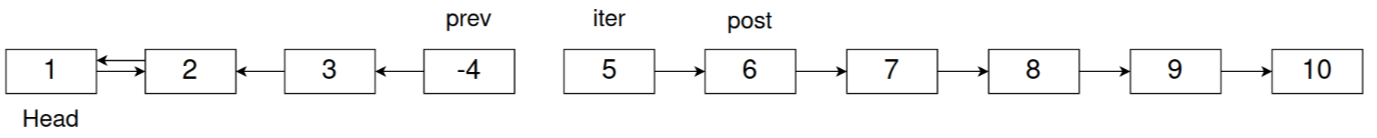
\includegraphics[width=\textwidth]{img/fig17.png}
  \end{figure}

\end{frame}

\begin{frame}
  \frametitle{Funcionamiento del algoritmo}

  Hacer que el nodo \cppinline{iter} apunte al nodo \cppinline{prev}

  \begin{figure}[h]
    \centering
    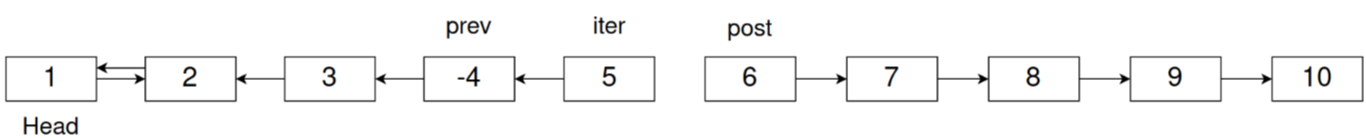
\includegraphics[width=\textwidth]{img/fig18.png}
  \end{figure}

  Mover \cppinline{prev} a \cppinline{iter}

  \begin{figure}[h]
    \centering
    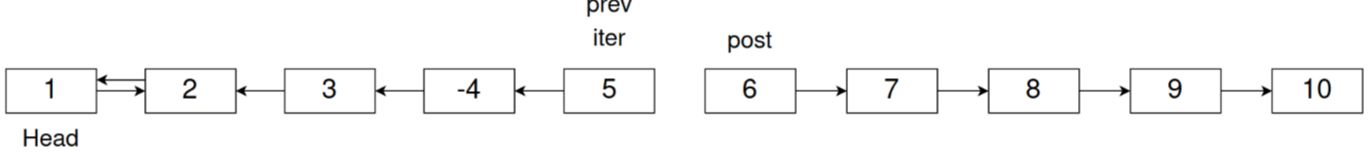
\includegraphics[width=\textwidth]{img/fig19.png}
  \end{figure}

\end{frame}

\begin{frame}
  \frametitle{Funcionamiento del algoritmo}

  Mover \cppinline{iter} a \cppinline{post}

  \begin{figure}[h]
    \centering
    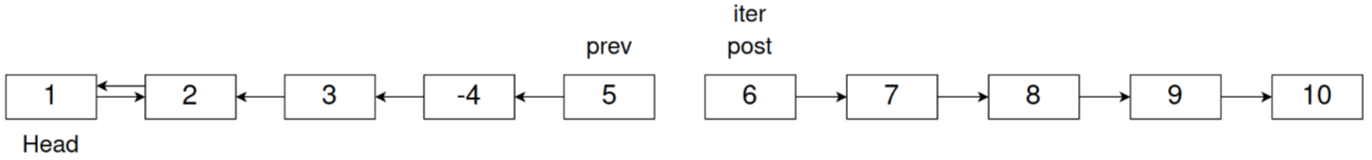
\includegraphics[width=\textwidth]{img/fig20.png}
  \end{figure}

  $i = 4$, condición $i < k-1$. $k = 5$. \textbf{Finaliza el ciclo}.

  \begin{figure}[h]
    \centering
    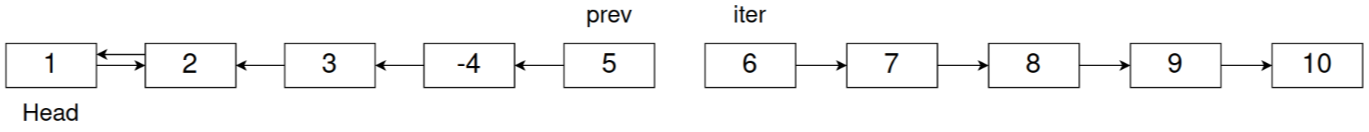
\includegraphics[width=\textwidth]{img/fig21.png}
  \end{figure}

\end{frame}

\begin{frame}
  \frametitle{Funcionamiento del algoritmo}

  Hacer que \cppinline{head} apunte a \cppinline{iter}.

  \begin{figure}[h]
    \centering
    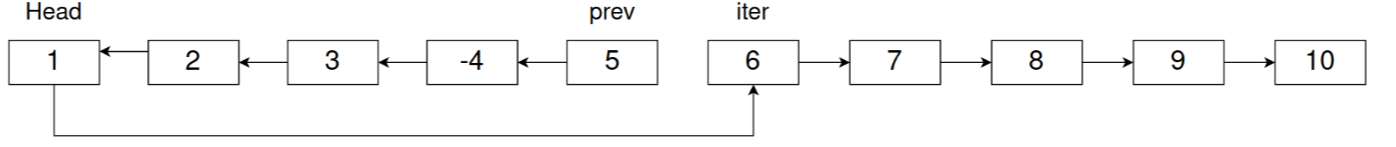
\includegraphics[width=\textwidth]{img/fig22.png}
  \end{figure}

  Hacer que \cppinline{head} sea \cppinline{prev}.

  \begin{figure}[h]
    \centering
    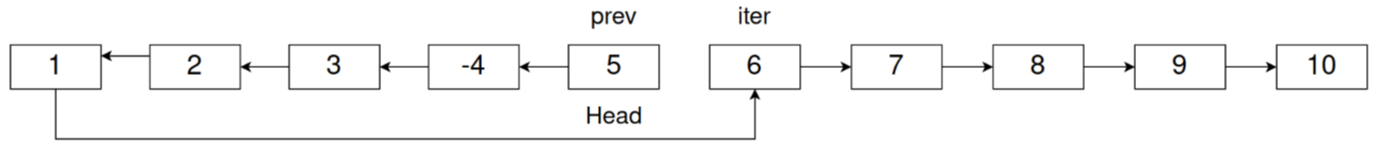
\includegraphics[width=\textwidth]{img/fig23.png}
  \end{figure}

\end{frame}

\begin{frame}
  \frametitle{Funcionamiento del algoritmo}

  La lista entonces se ve:

  \begin{figure}[h]
    \centering
    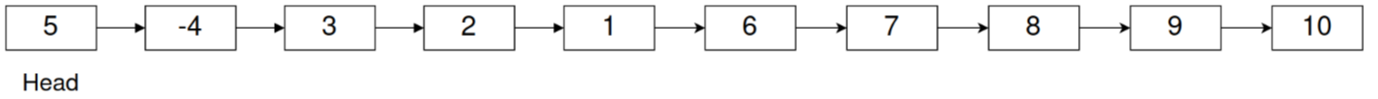
\includegraphics[width=\textwidth]{img/fig24.png}
  \end{figure}



\end{frame}



\section{Implementación En C++}

\insertsectionpage

\begin{frame}
  \frametitle{Implementación en C++}

 \scalebox{0.8}{\lstinputlisting[style=cppstyle]{SPPilasColasP2.cpp}}

\end{frame}

\section{Complejidad temporal y espacial}

\insertsectionpage

\begin{frame}
  \frametitle{Complejidad temporal y espacial}

  \begin{itemize}
    \item Mayoría de casos $O(k)$. Peor de los casos $k = n$
          \[
          O(n)
          \]
    \item Espacial, no se crean nuevas estructuras.
          \[O(1)\]
  \end{itemize}

\end{frame}



% \section{Referencias}

% \insertsectionpage
% \begin{frame}[allowframebreaks]{Referencias}
%   \printbibliography
% \end{frame}


\insertendpage

\end{document}
